\documentclass[letterpaper,twocolumn,10pt]{article}

\usepackage[utf8]{inputenc}
\usepackage[T1]{fontenc}
\usepackage{fouriernc}
\usepackage{amsmath}
\usepackage{amssymb}
\usepackage{amsthm}
\usepackage{booktabs}
\usepackage[labelfont=bf]{caption}
\usepackage{circuitikz}
\usepackage{enumitem}
\usepackage{float}
\usepackage{geometry}
\usepackage{graphicx}
\usepackage{hyperref}
\usepackage{mathtools}
\usepackage{microtype}
\usepackage{nicefrac}
\usepackage{pdfpages}
\usepackage{physics}
\usepackage{rotating}
\usepackage{siunitx}
\usepackage{xcolor}

\geometry{margin=1in}

\newcommand{\refdes}[1]{\texttt{#1}}
\newcommand{\wtemp}{\ensuremath{\blacklozenge}}

\renewcommand{\includepdf}{}

\title{Lab Power Supply Manual}
\author{Alex Striff}
\date{\today}

\begin{document}
\maketitle
\tableofcontents
\listoftables
\thispagestyle{empty}

\section*{Colophon}

The schematic diagram and printed circuit board layout were both created with
KiCAD. This manual was compiled using \LaTeX. Relatively fine (\SI{0.51}{\mm})
lead-based solder and mildly activated rosin flux were required to solder the
components to the PCB.

\section{Acknowledgments}

The creation of this lab power supply was generously funded by the Reed College
Physics Department. I would like to thank Edgar Perez for his kind advice, as
well as Lucas Illing for supporting this project.

\section{Motivation}

Often when working in electronics, several voltage sources are needed. In
addition to a main power rail, one may need a complementary negative power rail
for analog circuitry, or a different logic power supply at \SI{3.3}{\V} instead
of \SI{5}{\V}. Low-impedance bias voltages are also a frequent requirement,
needed for biasing BJTs, comparator inputs, and more.

For most applications, a power supply fulfilling the requirements of these
applications need not be capable of supplying much more than \SI{1}{\A} of
current, must have a stable voltage output (requiring a linear regulator), and
must have a current limiting function.  Additionally, it would be nice if the
power supply was much smaller than a conventional \SI{30}{\V}, \SI{3}{\A} output
bench power supply with a large transformer, being conveniently powered from a
common wall plug, batteries, or any other DC power source at hand. I have
attempted to construct such a power supply.

\section{Safety Notice (Grounding)}

Please note that the negative voltage output of the supply is directly connected
to the negative voltage input to the supply. That is, the output voltage of the
supply floating relative to earth ground if and only if the input voltage is
floating.

If you are uncertain if the supply (or any other piece of equipment) is
floating, it is quick and simple to check if this is the case. Set a digital
multimeter to its resistance measurement or continuity check mode. Connect one
probe to the negative output of the PSU (the black five-way binding post) or to
the other terminal in question, and then connect the other probe to earth
ground. This can be done either by insertion in to the \emph{earth} socket of a
wall outlet, or by touching the outside of a BNC connector on any nearby
oscilloscopes, as these are almost always earth grounded. If inserting into a
wall outlet, be certain that you know which hole is which, and that you are
using a multimeter approved for wall testing (most are).

If the output is not floating (earth-referenced), then one must be careful to
only connect oscilloscope ground leads to the negative output of the supply.
Whatever the ground lead is connected to will be shorted to earth ground. If an
incorrect connection is made, then connected circuit components, oscilloscopes,
or computers (\textit{e.g.} through USB) may be damaged. If you are uncertain,
connect probes as if the circuit is not floating.

If the output is floating (or if you know which terminals are earthed and which
are not), then the supply may be safely connected to other voltage sources in
whatever configurations are convenient, such as in a dual-rail setup.

\section{Usage Instructions}

\subsection{Setting the output voltage}

Connect a voltmeter to the output of the supply. You may use either the binding
posts or the test points labeled on the board to achieve this. Turn the PSU on
and adjust the voltage using the \emph{coarse} and \emph{fine} adjustment knobs
as needed. Note that the maximum output voltage is about \SI{1.5}{\V} below the
input voltage.

\subsection{Setting the current limit}\label{sec:set_limit}

To set the current limit to its minimum value, \emph{short} the minimum limit
jumper (labeled \emph{Min Lim}, \refdes{JP1}). To set the current limit to
higher than this value, the jumper must be \emph{open}.

The current limit is set to fixed values by moving the switches on the
board. The default values are 1, 2.5, 5, 10, 25, 50, and \SI{100}{\mA}. To set
the limit to any of the upper four values, the switch for the lower values must
be in its rightmost position, as indicated on the board.

Alternatively, the switch section on the board may not be populated, and a
\SI{10}{\kohm} (preferably 10-turn) potentiometer (\refdes{RV4}) may be
soldered in to provide a continuously variable current limit.

To set the current limit to its maximum value, \emph{open} the no limit jumper
(labeled \emph{No Limit}, \refdes{JP2}). To set the current limit to lower than
this value, the jumper must be \emph{shorted}. The maximum value is about
\SI{2.0}{\A} in normal operation, and less when the device shuts down to prevent
overheating.

\subsection{Indicator LEDs}

The power supply includes two indicator LEDs for when output voltage regulation
is not guaranteed.

The \textit{Hot} indicator LED (\refdes{D2}) lights when the main regulation IC
(see Section~\ref{sec:lt3081}) starts to get hot (when the junction temperature
is about \SI{100}{\celsius} or above). This light is a warning, and the output
should continue to be regulated as normal. If the IC continues to heat up (to a
junction temperature of \SI{125}{\celsius}), then internal protection circuitry
will prevent damage and reduce the output voltage.

The \textit{$V_\text{out}$ Error ($I$ lim)} indicator LED (\refdes{D1}) lights
when the actual output voltage is not sufficiently close to the set output
voltage. The most common cause for this is if the current limiting function is
active, but internal protection circuitry or a set voltage that is too high may
also cause an output error.

\subsection{Monitoring the output current}

If it is not preferred to use an ammeter to measure the output current, the
\textit{$I_\text{out}$} test point is provided for convenient measurement or
external control of the load current. The signal at \textit{$I_\text{out}$}
is one volt for every ampere of output current, \emph{including the internal
load} (see Table~\ref{tab:chars} and Section~\ref{sec:int_load}). For example,
if the supply is outputting \SI{25}{\mA} total, then \textit{$I_\text{out}$}
should read \SI{25}{\mV}.

\subsection{Monitoring the internal temperature}

For more quantitative information about the temperature of the main regulation
IC (see Section~\ref{sec:lt3081}) than is provided by the \textit{Hot} indicator
LED, the \textit{Temp} test point is provided. The signal at \textit{Temp} is
one millivolt for every degree Celsius of junction temperature. For example, if
the junction temperature of the IC is about \SI{73}{\celsius} (subject to
variation inside the IC), then \textit{Temp} should read \SI{73}{\mV}.

\subsection{Disabling the internal load}

The internal load may be disabled by \emph{opening} the \textit{Internal Load}
jumper.  Note that this will increase the current limit by at most \SI{4}{\mA}
above the current limit displayed on the switches or that previously set by
\refdes{RV4}, if installed. For most purposes, the \textit{Internal Load} jumper
should be in its normal, \emph{shorted} position (see
Section~\ref{sec:int_load}).

\subsection{Calibrating the current limit}

The power supply requires a minimum load in order to regulate the output voltage
properly. An internal load usually supplies this minimum load (see
Section~\ref{sec:int_load}), but this offsets the effective current limit on the
output. A trimmer potentiometer is provided to compensate for this offset.

Set the supply to the minimum limit as described in Section~\ref{sec:set_limit}.
Using a screwdriver, adjust the potentiometer (labeled \emph{Load
Offset}, \refdes{RV1}) until the output voltage is stable (no current limiting),
and then carefully reverse direction and adjust until the current limit just
starts to activate. This may be judged by checking the output voltage with a
voltmeter, or by using the built-in indicator if it is calibrated as described
in Section~\ref{sec:cal_offset}

\subsection{Calibrating the output error indicator}\label{sec:cal_offset}

The issues associated with creating a reliable output error indicator are
discussed in Section~\ref{sec:how_offset}. If necessary, a trimmer potentiometer
(\refdes{RV5}) may be populated to correct the default setting by the resistor
\refdes{R21}.

Attach a voltmeter to the PSU and set the output voltage to \SI{1}{\V}. Attach
an external potentiometer to the output of the supply, valued to draw a typical
current for your application. Set the PSU current limit so that increasing the
load current will trigger the limit function. If the \SI{1}{\V} output does not
demand enough current, it may be increased, but try to keep it as low as
possible (see \ref{sec:how_offset} for why). Wait until the temperature of the
circuit has stabilized. Error on the side of drawing a slightly lower current
than needed, depending on the sensitivity required (see below). Increase the
load gradually, and watch the error indicator LED (\refdes{D1}).

If the default indication threshold set by \refdes{R21} is not sensitive enough
for your needs, solder in the \SI{500}{\kohm} \refdes{RV5} and try the
adjustment procedure below.

If this does not work, or if the default indication did not work at all, solder
in \refdes{RV5} and \emph{remove} \refdes{R21}. This provides a wider range of
variation for the indication threshold, at the cost of a coarser adjustment
rate.

With the potentiometer \refdes{RV5} and the default resistor \refdes{R21}
soldered on the board or not depending on your needs, adjust the external load
potentiometer until the output is 2 -- \SI{10}{\mV} below the set voltage. If
you intend to use the supply \emph{only} above about \SI{5}{\V}, the lower the
better (you may even be able to remove \refdes{RV5} and wire a short across
\refdes{R21} for a bit more sensitivity). To complete the calibration, adjust
\refdes{RV5} to the barrier where \refdes{D1} just barely lights, or perhaps
flickers.

% \section{Electrical Characteristics}

\begin{table*}[ht]
  \centering
  \caption[Electrical Characteristics]{Electrical characteristics. The \wtemp\
    mark indicates specifications which apply over the full operating
    temperature range. Otherwise, specifications are at (junction) temperatures
  of \SI{25}{\celsius}.}
  \resizebox{\textwidth}{!}{%
    \begin{tabular}{lr|lr|cccr}
      \toprule
      \multicolumn{2}{c}{\textbf{Parameter}} &
      \multicolumn{2}{c}{\textbf{Conditions}} & \textbf{Min} & \textbf{Typ} &
      \textbf{Max} & \multicolumn{1}{c}{\textbf{Units}} \\
      \midrule
      Input Voltage & $V_\text{in}$ & & \wtemp & 5.0 & & 32.0 & \si{\V} \\

      Output Voltage & $V_\text{out}$
      & $I_\text{load} < I_\text{lim}$ & \wtemp
      & 0.0 & & $V_\text{in} - V_\text{do}$ & \si{\V} \\

      Dropout Voltage & $V_\text{do}$
      & $I_\text{load} = \SI{100}{\mA}$ & & & 1.21 & & \si{\V} \\
      &
      & $I_\text{load} = \SI{1.5}{\A}$ & \wtemp & & 1.23 & 1.5 & \si{\V} \\

      Internal Current Limit & $I_\text{max}$ & $V_\text{in} = \SI{5}{\V}$,
      $V_\text{set} = \SI{0}{\V}$, $V_\text{out} = \SI{-0.1}{\V}$ & \wtemp
      & 1.5 & 2.0 & & \si{\A} \\

      $I_\text{out}$ Relative Error & & $I_\text{load} = \SI{1.5}{\A}$ &
      & 0 & 6 & 11 & \si{\percent} \\

      $I_\text{out}$ Operating Range & & & \wtemp
      & $V_\text{out} - \SI{40}{\V}$ & & $V_\text{out} + \SI{0.4}{\V}$
      & \si{\V} \\

      \textit{Temp} Absolute Error &
      & $\SI{0}{\celsius} \le T_J \le \SI{125}{\celsius}$ &
      & -10 & & 10 & \si{\uA} \\
      &
      & $\SI{125}{\celsius} < T_J \le \SI{150}{\celsius}$ &
      & -15 & & 15 & \si{\uA} \\

      Ripple Rejection
      & PSRR & $f = \SI{120}{\Hz}$ & & 75 & 90 & & \si{\dB} \\

      $V_\text{ripple} = \SI{0.5}{V_{\text{pp}}}$,
      $I_\text{load} = \SI{0.1}{\A}$, &
      & $f = \SI{10}{\kHz}$ & & & 75 & & \si{\dB} \\

      $V_\text{in} = V_\text{out(nom)} + \SI{3}{\V}$ &
      & $f = \SI{1}{\MHz}$ & & & 20 & & \si{\dB} \\

      Internal Load & $I_\text{int}$ & & \wtemp & 2 & 3 & 4 & \si{\mA} \\
      \bottomrule
  \end{tabular}}
  \label{tab:chars}
\end{table*}
\clearpage

\section{Principles of Operation}

\subsection{The LT3081 linear regulator}\label{sec:lt3081}

All of the regulation that the power supply provides is done by the LT3081, a
rugged linear regulator IC. The regulation circuitry is depicted in
Figure~\ref{fig:reg_circ}. An internal current source of \SI{50}{\uA} allows the
set voltage to be configured with a single resistor $R_\text{set}$. In the power
supply, $R_\text{set}$ is determined by the two potentiometers \refdes{RV2} and
\refdes{RV3}.

If $V_\text{out} < V_\text{set}$, then the error amplifier will increase the
base voltage of the NPN transistor until the entire Sziklai pair has
$V_\text{set}$ at its emitter. Similarly, the base voltage will be suitably
reduced if $V_\text{out} > V_\text{set}$. In this way, the output voltage is
regulated by a negative feedback loop.

In practice, it may be difficult to stabilize such a circuit constructed of
discrete components against oscillation. Using an integrated circuit solution
such as the LT3081 allows us to have matched transistors at close to the same
temperature, as well as to take advantage of the work done by previous engineers
to make the output voltage stable. We simply add on some additional capacitances
(\refdes{C1} to \refdes{C4} and \refdes{C8}) to improve noise characteristics,
transcient performance, and stability a bit more.

\begin{figure}
  \centering
  \begin{circuitikz} \draw
    (0,0) node[op amp,yscale=-1] (opamp) {}
    (-3,0.5) to [short] (opamp.+)
    (-3,2.5) to [short,-o] (3.5,2.5)
    node[anchor=west]{$V_{\text{in}}$} (vin)
    (-3,2.5) to [american current source,l=\SI{50}{\uA}] (-3,0.5)
    (-3,0.5) to [R,l=$R_\text{set}$,*-] (-3,-1.5)
    node [ground] {}
    (opamp.out) node[npn,anchor=B] (npn) {} (npn.collector)
    (npn.collector) node[pnp,anchor=B] (pnp) {} (pnp.collector)
    (pnp.collector) to [short,-*] ($(pnp.collector)+(0,-1.5))
    (pnp.emitter) to [short,-*] ($(pnp.emitter)+(0,0.9625))
    (opamp.-) to [short] ($(opamp.-)+(0,-1))
    to [short,-o] (3.5,-1.5) node[anchor=west]{$V_\text{out}$}
    (npn.emitter) to [short,-*] ($(npn.emitter)+(0,-0.725));
  \end{circuitikz}
  \caption{The equivalent voltage regulation circuitry inside the LT3081. The
    equivalent current regulation circuitry is not depicted here or in the
  LT3081 datasheet.}
  \label{fig:reg_circ}
\end{figure}

\subsection{The internal load}\label{sec:int_load}

Given the requirement that any circuitry used in the power supply must function
consistently over the entire range of $V_\text{in}$, a simple resistor (as in
the LT3081 datasheet) \emph{cannot} be used as a means of meeting the minimum
load requirement of the LT3081. Instead, the LM334 current source (\refdes{U4})
was used. With \refdes{R23} set to \SI{22}{\ohm}, we expect about \SI{3.1}{\mA}
to be sunk from the output of the power supply, which is well above the minimum
load requirement of the LM3081, over temperature. Since we are manually nulling
the offset due to this current, it is allowable to use a common through-hole
\SI{5}{\percent} tolerance resistor for \refdes{R23}, but if your application
requires precise current limiting over a wide and changing range of
temperatures, a \SI{1}{\percent} or better tolerance resistor should be used for
added thermal stability.

\subsection{The \textit{Hot} indicator circuit}\label{sec:how_hot}

To establish a precise voltage of \SI{100}{\mV} over the entire range of
$V_\text{in}$, corresponding to a junction temperature of \SI{100}{\celsius}, a
\SI{2.5}{\V} LM4040 voltage reference (\refdes{U1}) and a voltage divider were
used. The LM393 comparator (\refdes{U3B}) compares the \textit{Temp} output to
this reference temperature, and is configured to pull the open collector output
of the comparator low if the \textit{Temp} output goes above the reference. This
connects the indicator LED to ground. A LM317 (\refdes{U6}) configured as a
current source supplies a stable current to the LED over the full range of
$V_\text{in}$. Inspection of the circuit shows that errors introduced by
resistor tolerances and comparator input offset currents and voltages will
result in an absolute error of at most \SI{5}{\celsius}. Furthermore, the
comparator operates without hysteresis, so the LED may flicker when the
actual and reference temperatures coincide. For the purpose of a coarse
temperature indication, these undesirable characteristics are inconsequential.

\subsection{The $V_\text{out}$ error indicator circuit}\label{sec:how_offset}

The general configuration of the $V_\text{out}$ error indicator circuit is
similar to that of the \textit{Hot} indicator circuit, described in
Section~\ref{sec:how_hot}. However, the error introduced by that circuit is
unacceptable for the purpose of displaying the current status of regulation.
Additionally, we \emph{expect} the output voltage to coincide \emph{precisely}
(to within a few millivolts) with the set voltage. Without any correction, the
LED may reasonably indicate an error indefinitely, or at least flicker, when the
output voltage is actually well-regulated.

The standard solution that one may propose is to add hysteresis (in the form of
a Schmitt trigger) to the comparator. This will not work. A Schmitt trigger must
have an upper trigger threshold that lies \emph{above} the set voltage, but in
the course of recovering from current limiting, the output voltage may never
overshoot the set voltage. Thus the threshold will never be crossed, and the
error indicator may remain on indefinitely. What is needed instead, is a small
offset.

If the comparator recieved a set voltage that was, say, \SI{10}{\mV} below
$V_\text{set}$, then the problem is solved. Hysteresis is not even needed, since
most all causes for a failure in regulation will not manifest as a steady offset
of \SI{10}{\mV}. But how can we create such a small offset over the entire range
of $V_\text{out}$, especially when the offset is comparable in size to all of
the sources of error involved? The main barriers to control that must be
addressed include
\begin{itemize}
  \item Resistor tolerances,
  \item Loading of input sources,
  \item Comparator input offset voltage,
  \item Comparator input bias current,
  \item Comparator input offset current, and
  \item Noise.
\end{itemize}

Since the entire point of adding the offset is to allow for errors, we can deal
with the comparator input offset voltage and current by lumping in the effect of
their worst-case absolute errors with the error in regulation. This increases
the minimum offset needed from that due to regulation, but only to about the
\SI{10}{\mV} stated before. However, we cannot increase the offset too much: at
an output voltage of \SI{1.00}{\V}, an offset of \SI{10}{\mV} already represents
a \SI{1}{\percent} error in indication. The aim is to keep this level of
precision for set voltages from \SI{1.00}{\V} to \SI{30.0}{\V}.

\clearpage
% \section{Schematic Diagram}

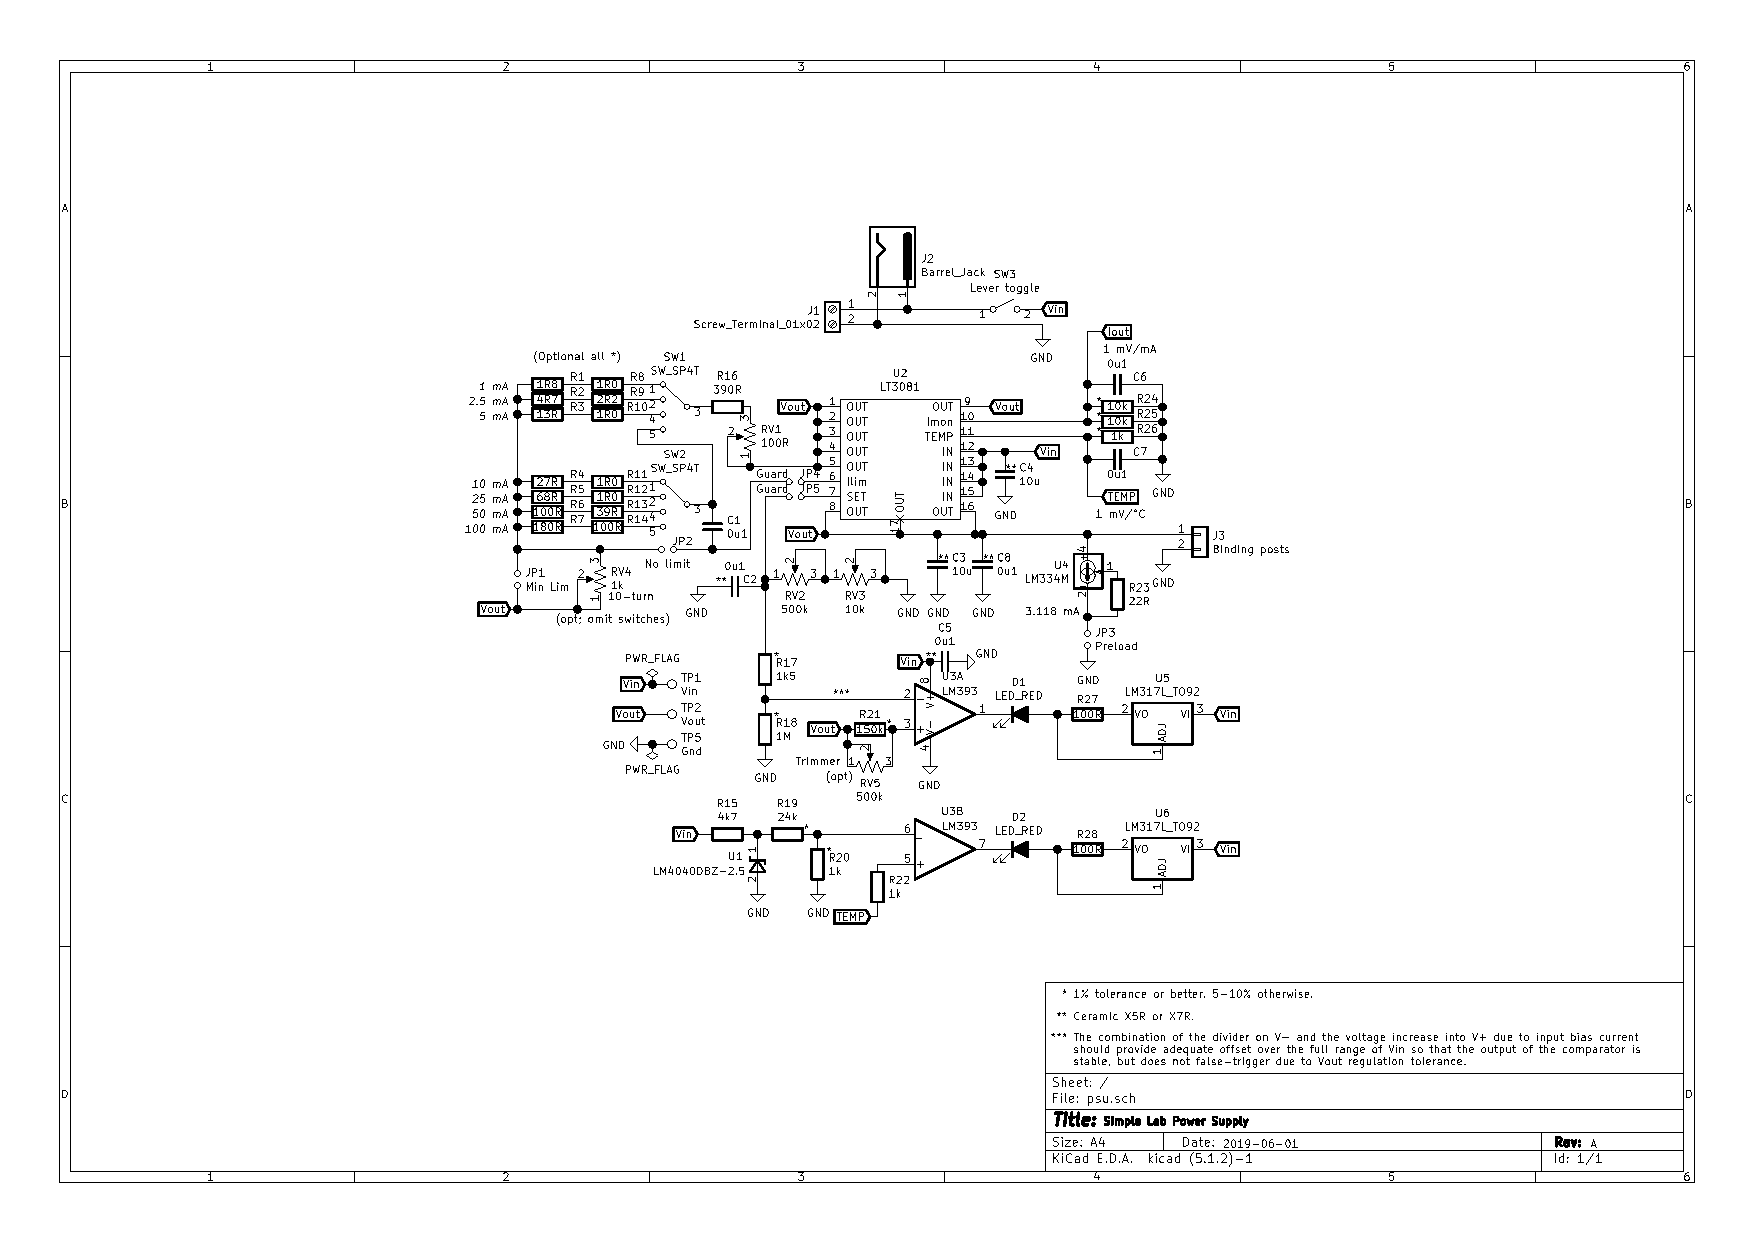
\includepdf[pages=-,pagecommand={},angle=90,addtotoc={1,section,1,Schematic
Diagram,fig:schematic}]{../psu-schematic.pdf}

\section{Printed Circuit Board Layers}

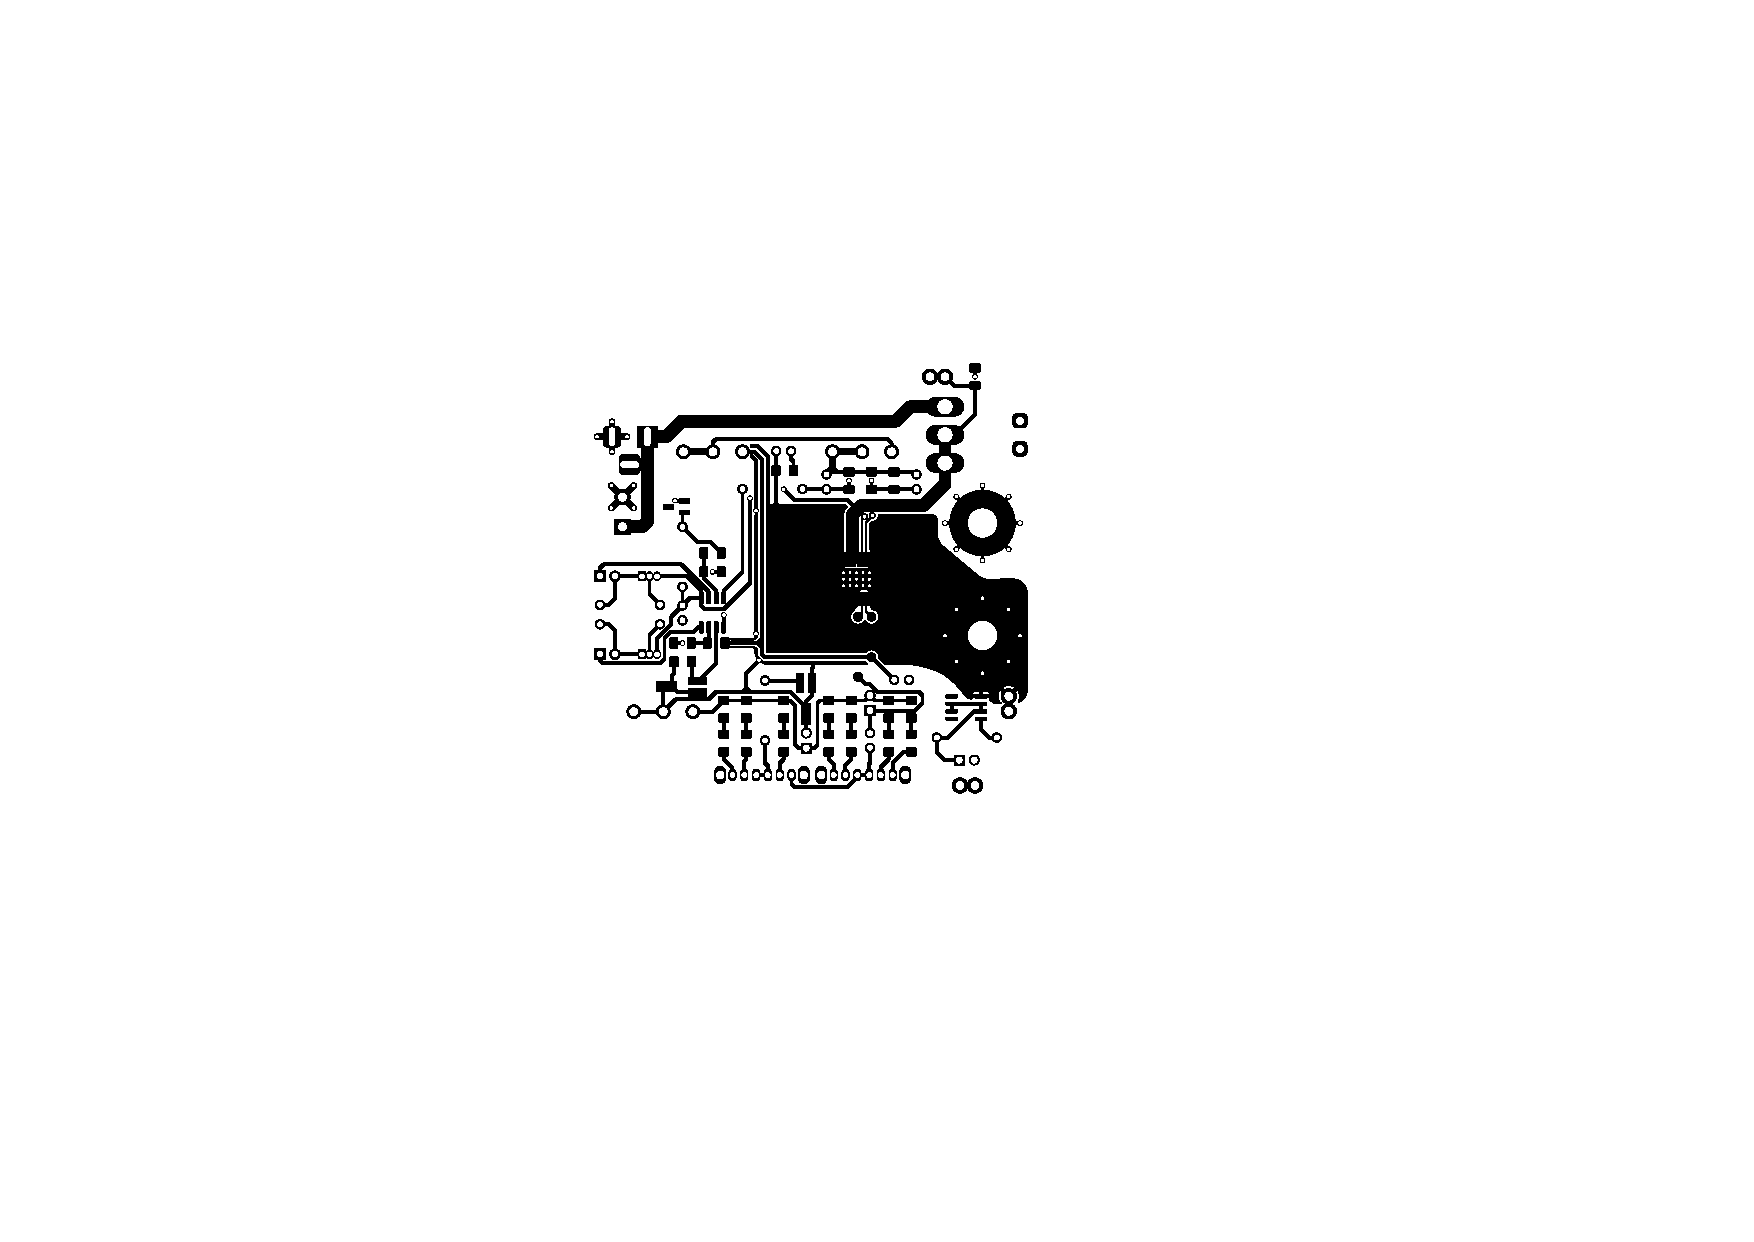
\includepdf[pages=-,pagecommand={},noautoscale=true,angle=90,addtotoc={1,subsection,2,Front
    Copper,fig:psu-F_Cu}]{../pcb/psu-F_Cu.pdf}
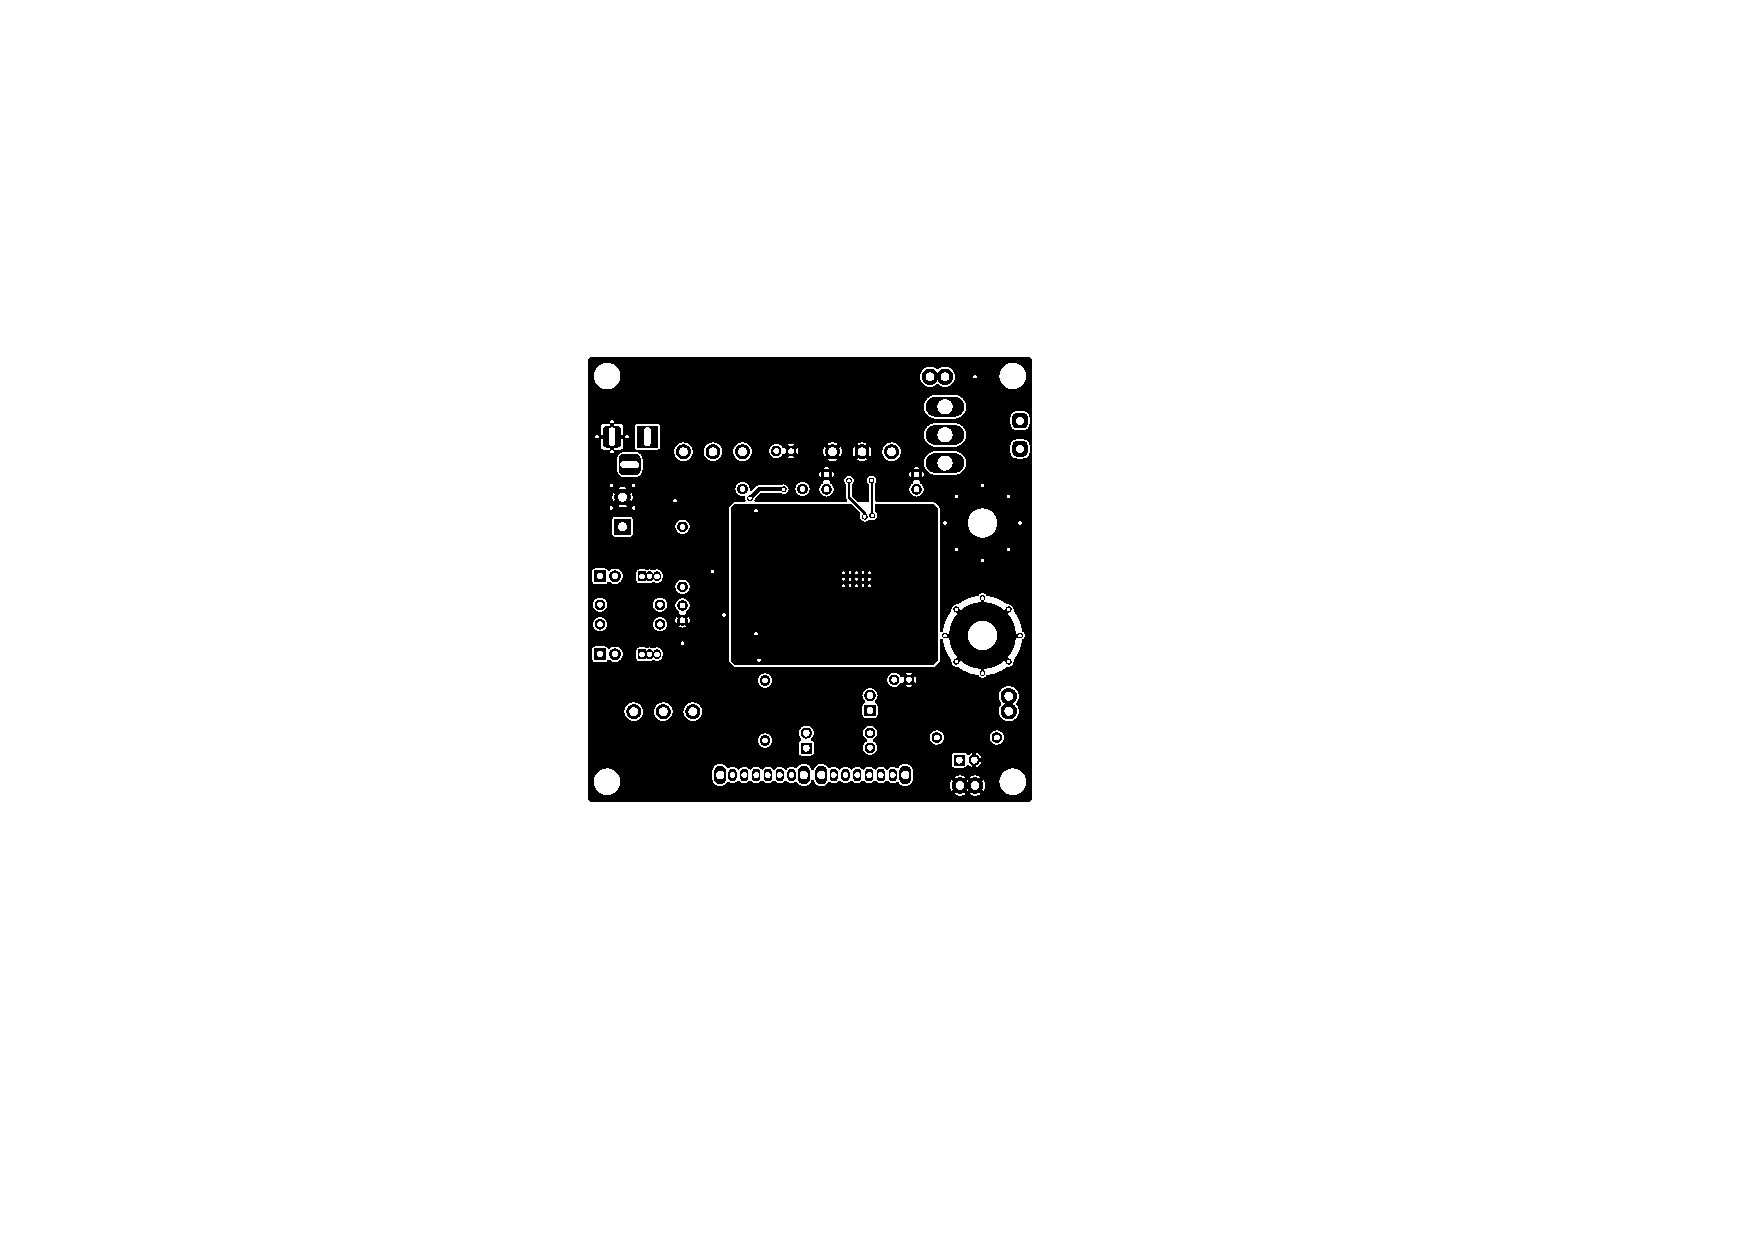
\includepdf[pages=-,pagecommand={},noautoscale=true,angle=90,addtotoc={1,subsection,2,Back
    Copper,fig:psu-B_Cu}]{../pcb/psu-B_Cu.pdf}
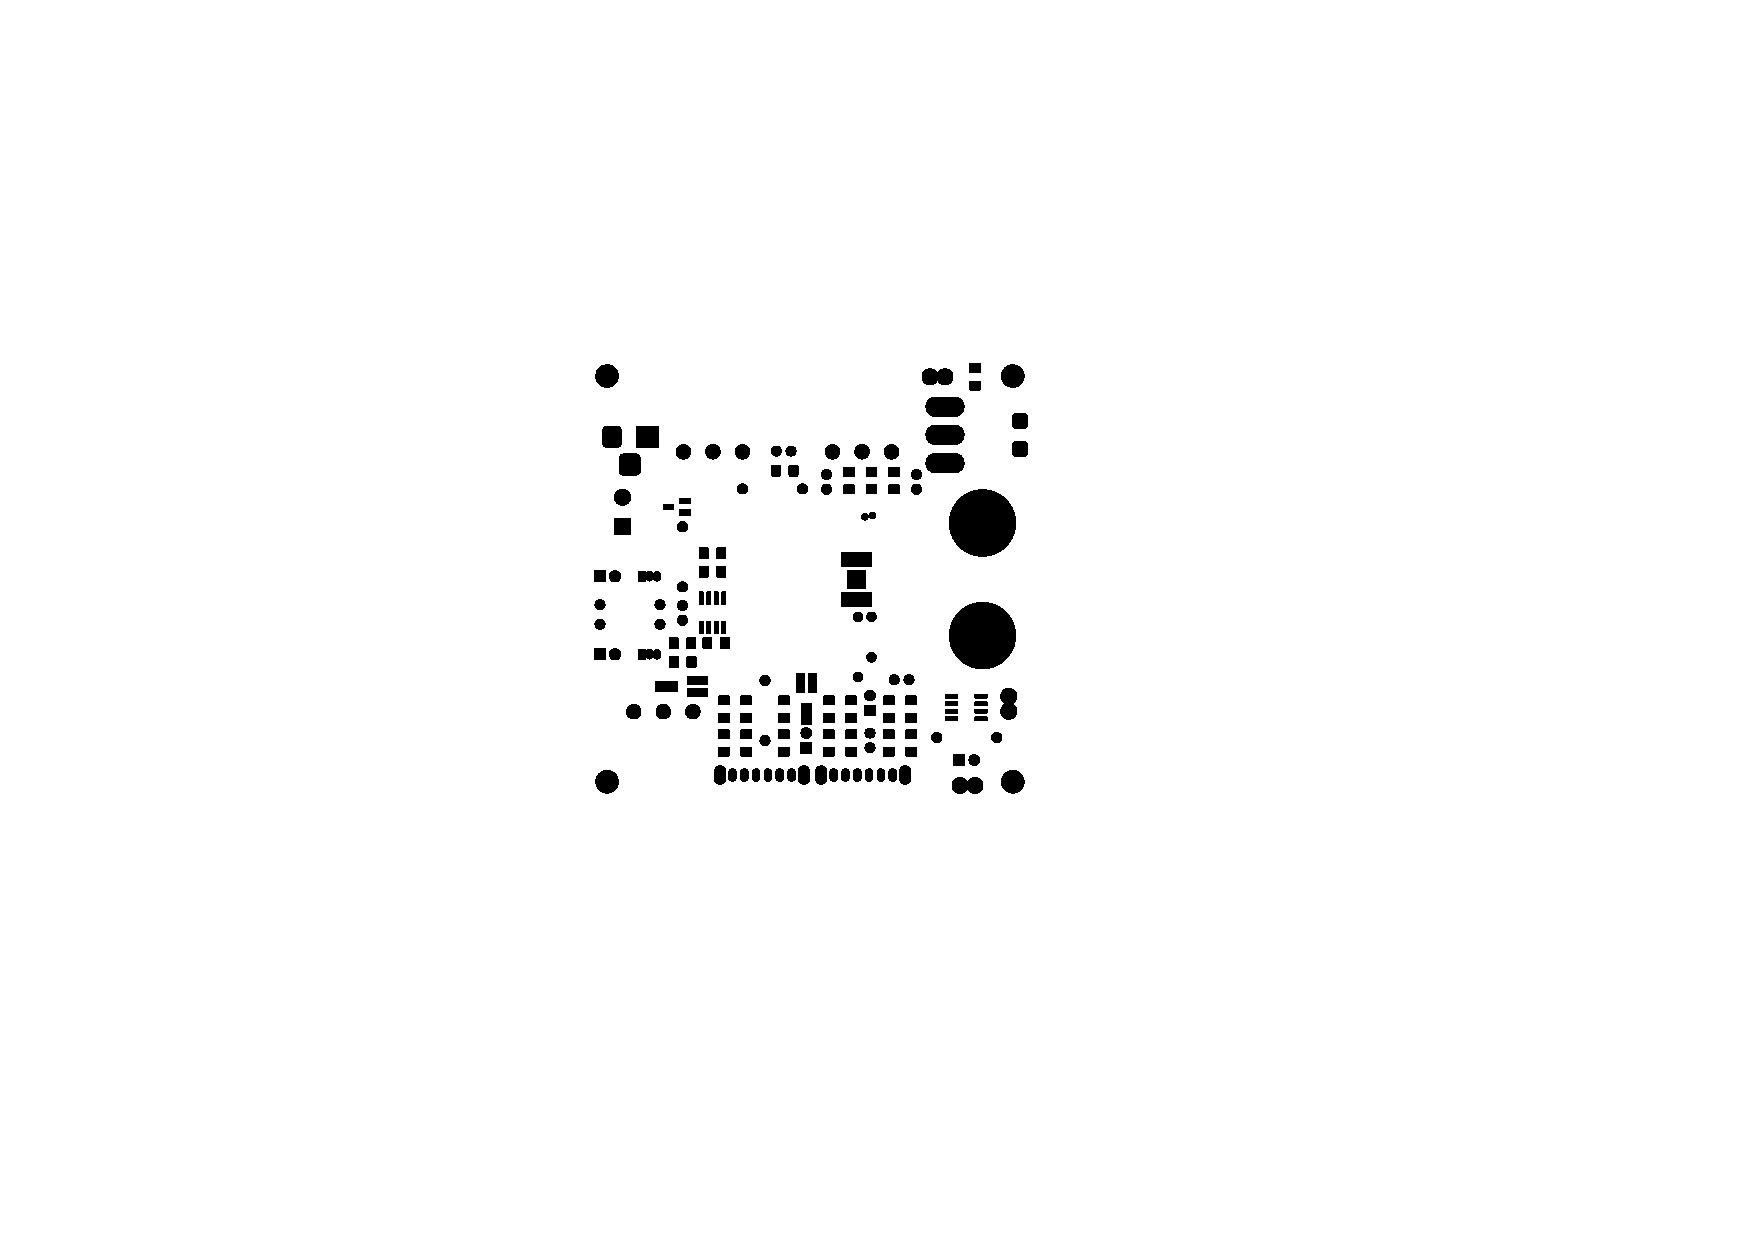
\includepdf[pages=-,pagecommand={},noautoscale=true,angle=90,addtotoc={1,subsection,2,Front
    Solder Mask,fig:psu-F_Mask}]{../pcb/psu-F_Mask.pdf}
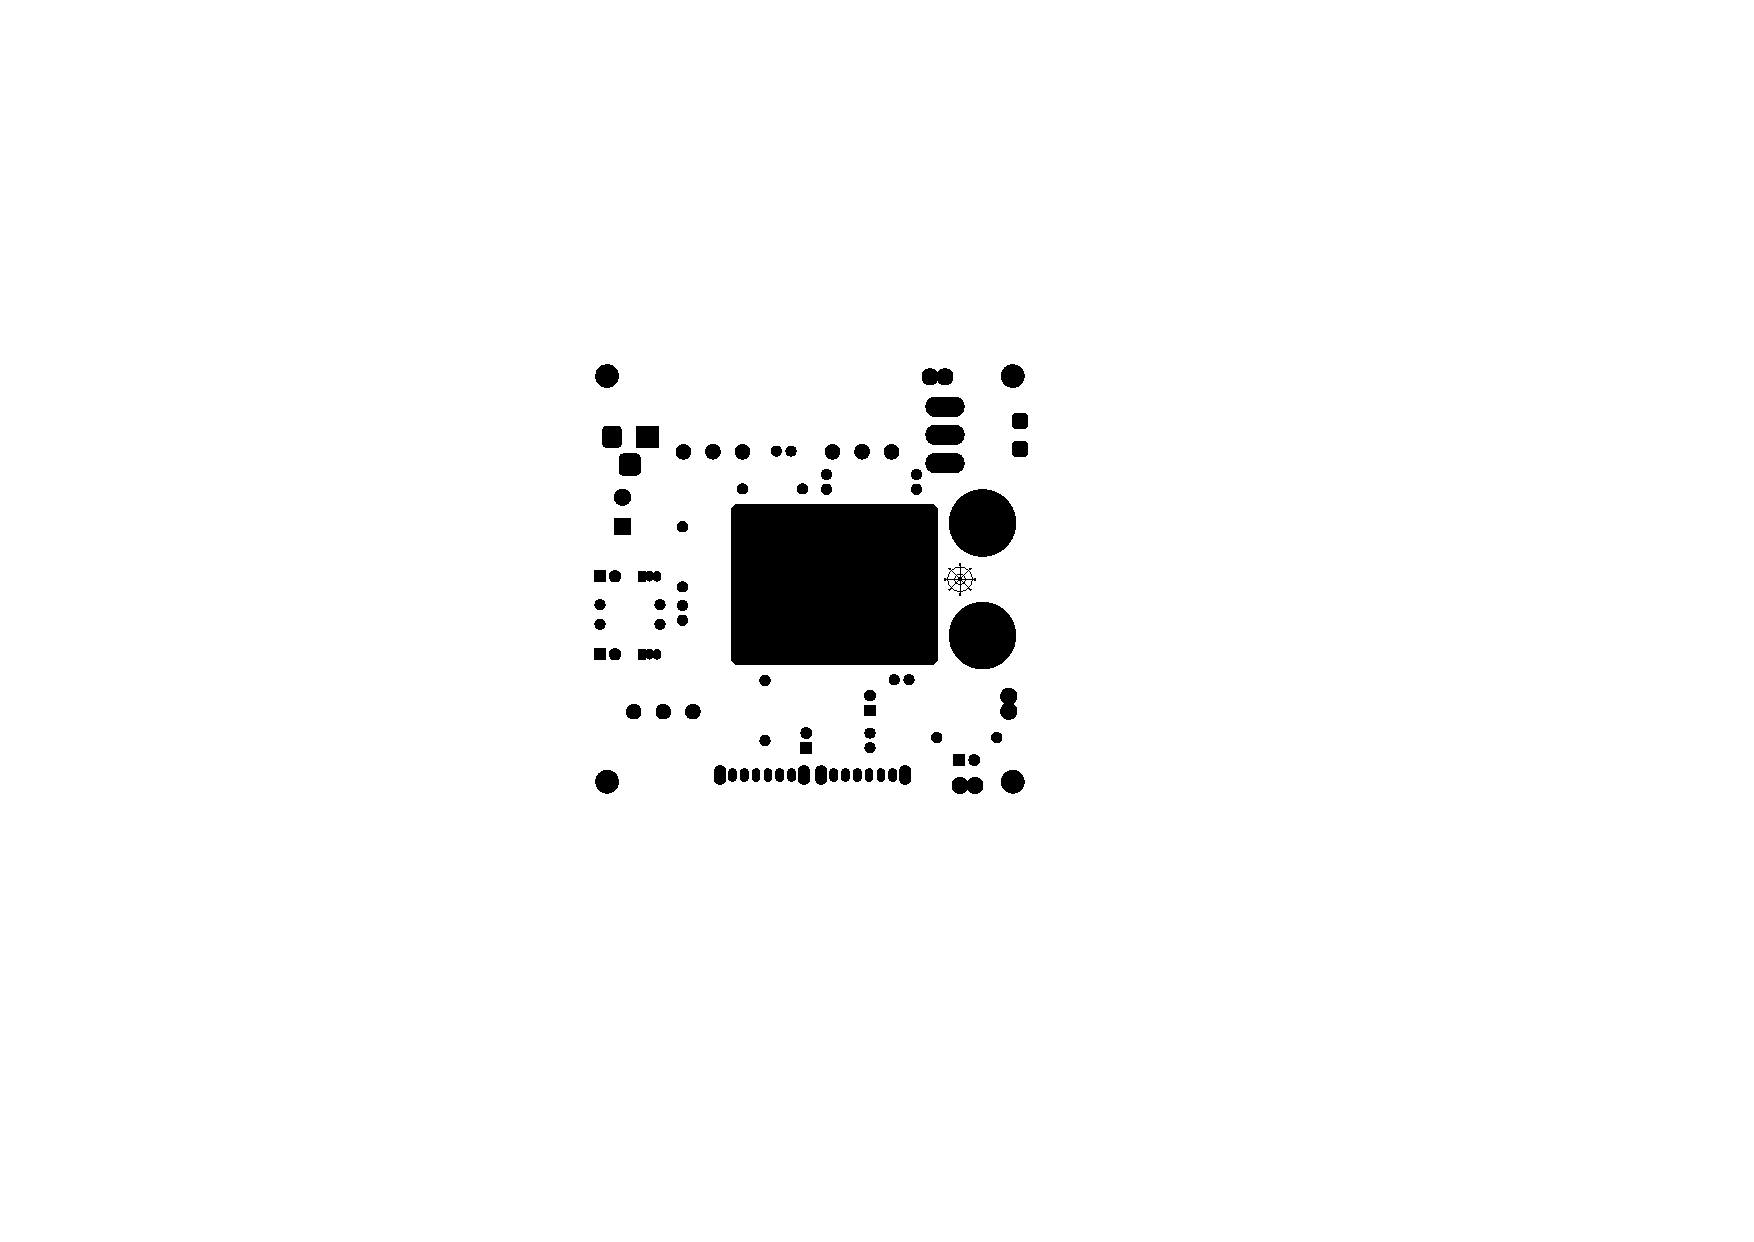
\includepdf[pages=-,pagecommand={},noautoscale=true,angle=90,addtotoc={1,subsection,2,Back
    Solder Mask,fig:psu-B_Mask}]{../pcb/psu-B_Mask.pdf}
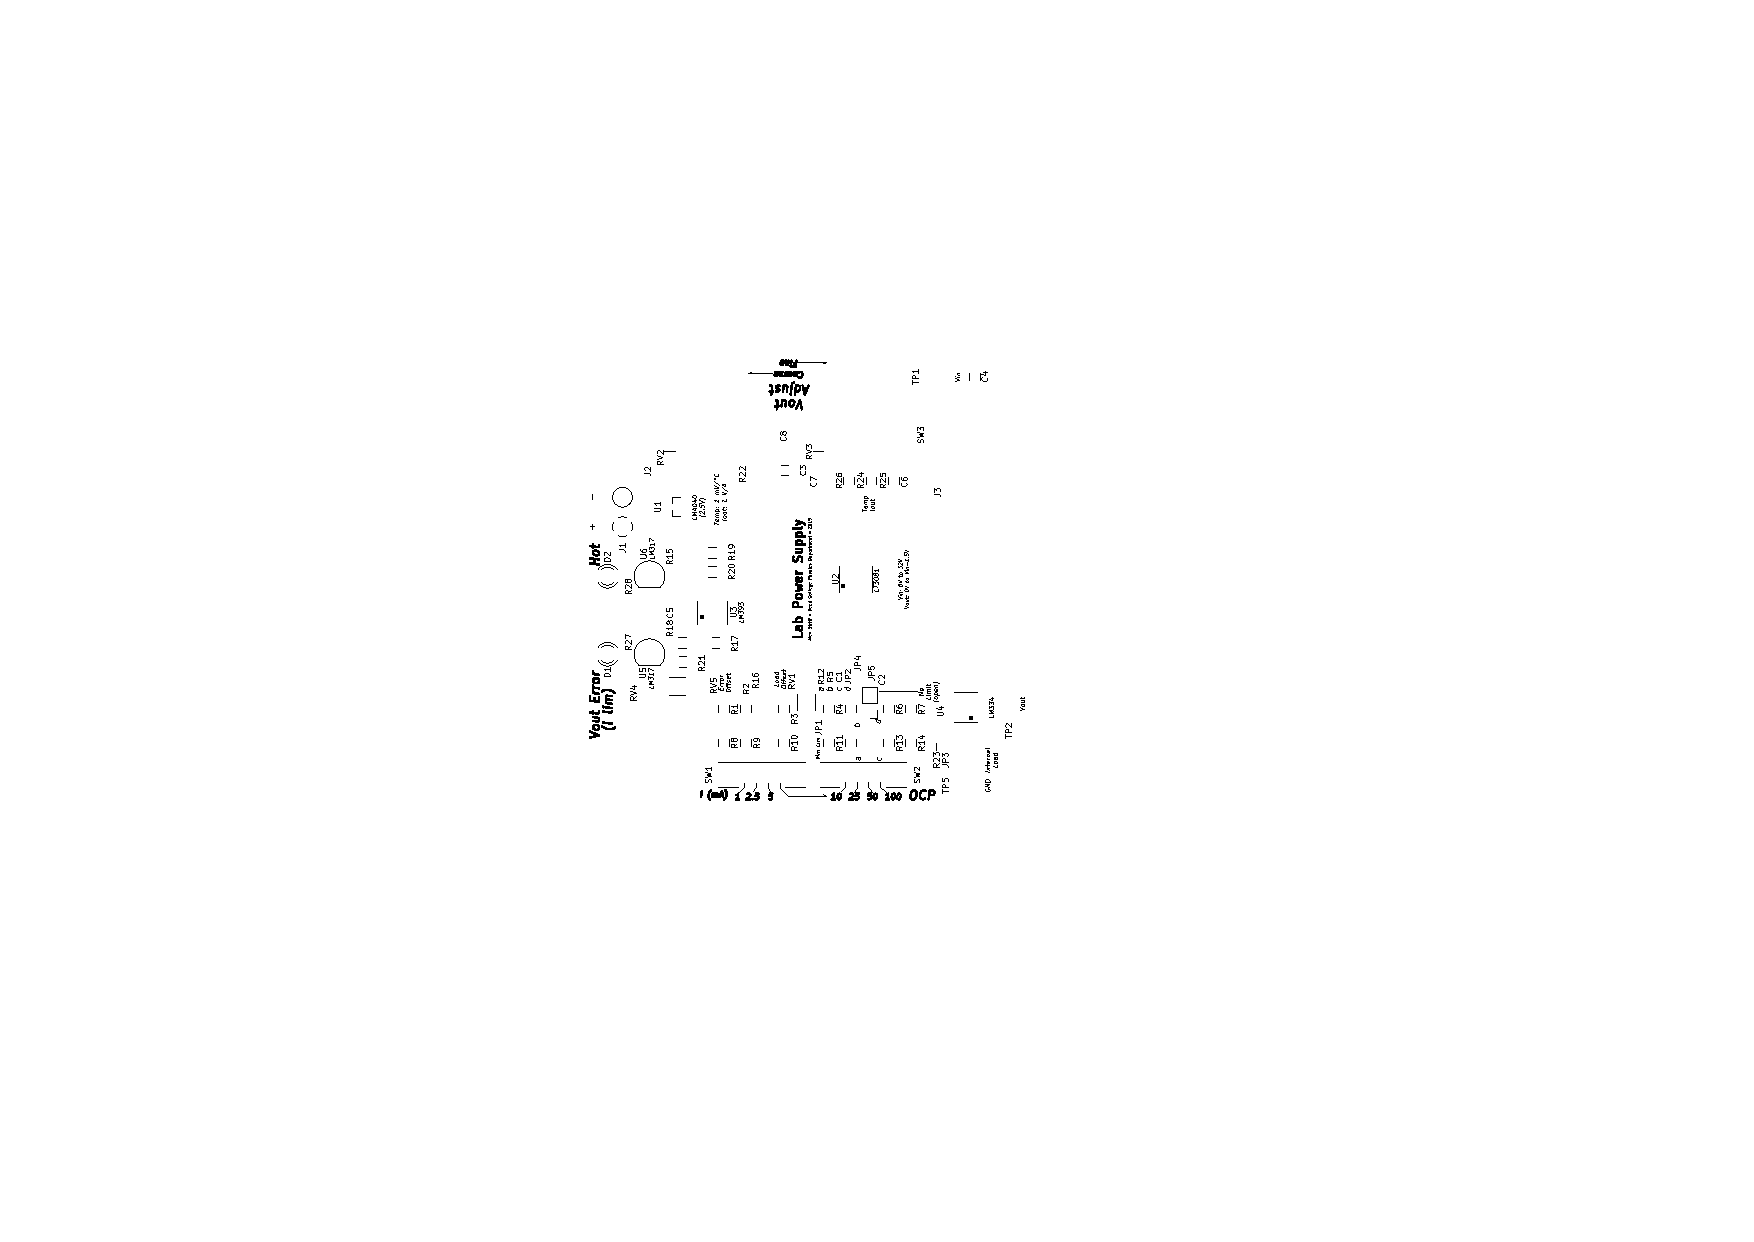
\includepdf[pages=-,pagecommand={},noautoscale=true,angle=90,addtotoc={1,subsection,2,Front
    Silk Screen,fig:psu-F_SilkS}]{../pcb/psu-F_SilkS.pdf}
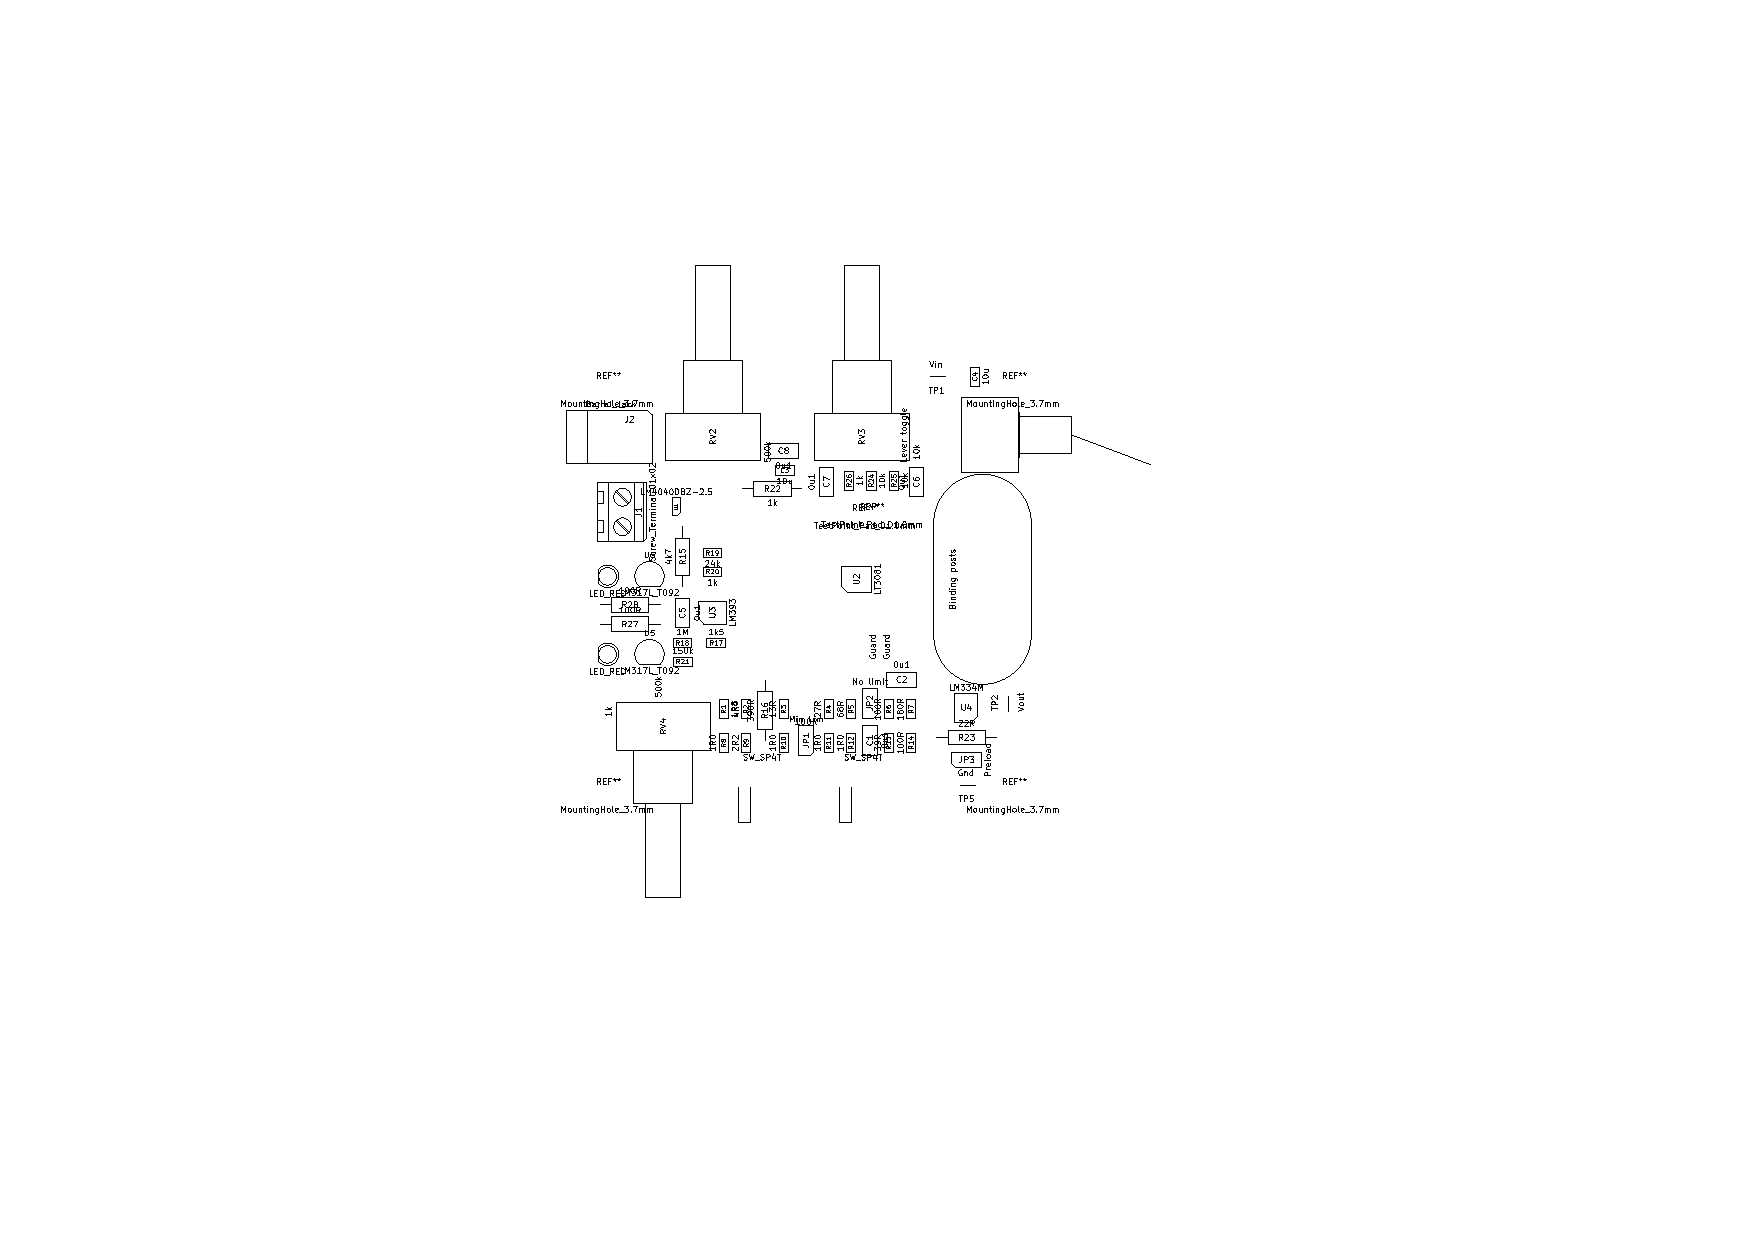
\includepdf[pages=-,pagecommand={},noautoscale=true,angle=90,addtotoc={1,subsection,2,Front
    Fabrication,fig:psu-F_Fab}]{../pcb/psu-F_Fab.pdf}
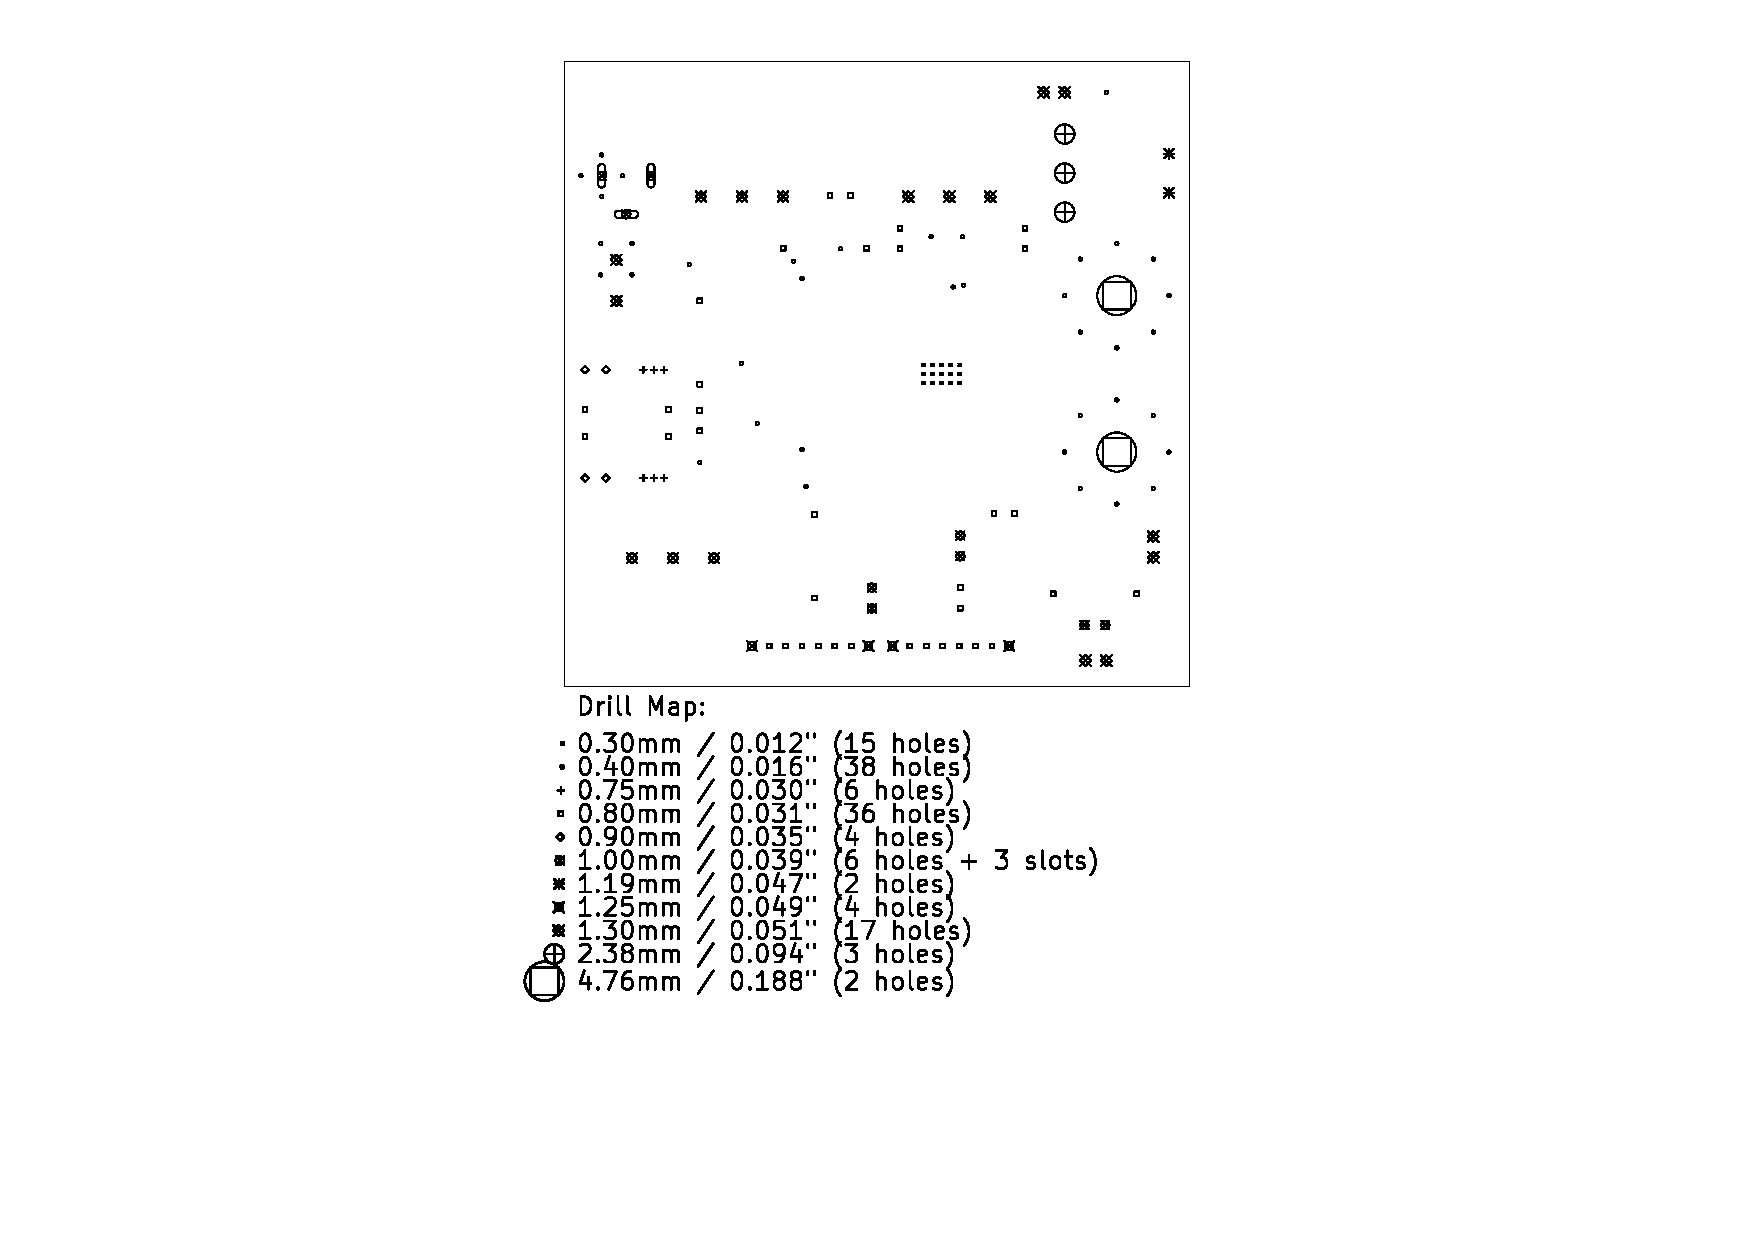
\includepdf[pages=-,pagecommand={},noautoscale=true,angle=90,addtotoc={1,subsection,2,Plated
    Through-Hole Drill Map,fig:psu-PTH-drl_map}]{../pcb/psu-PTH-drl_map.pdf}
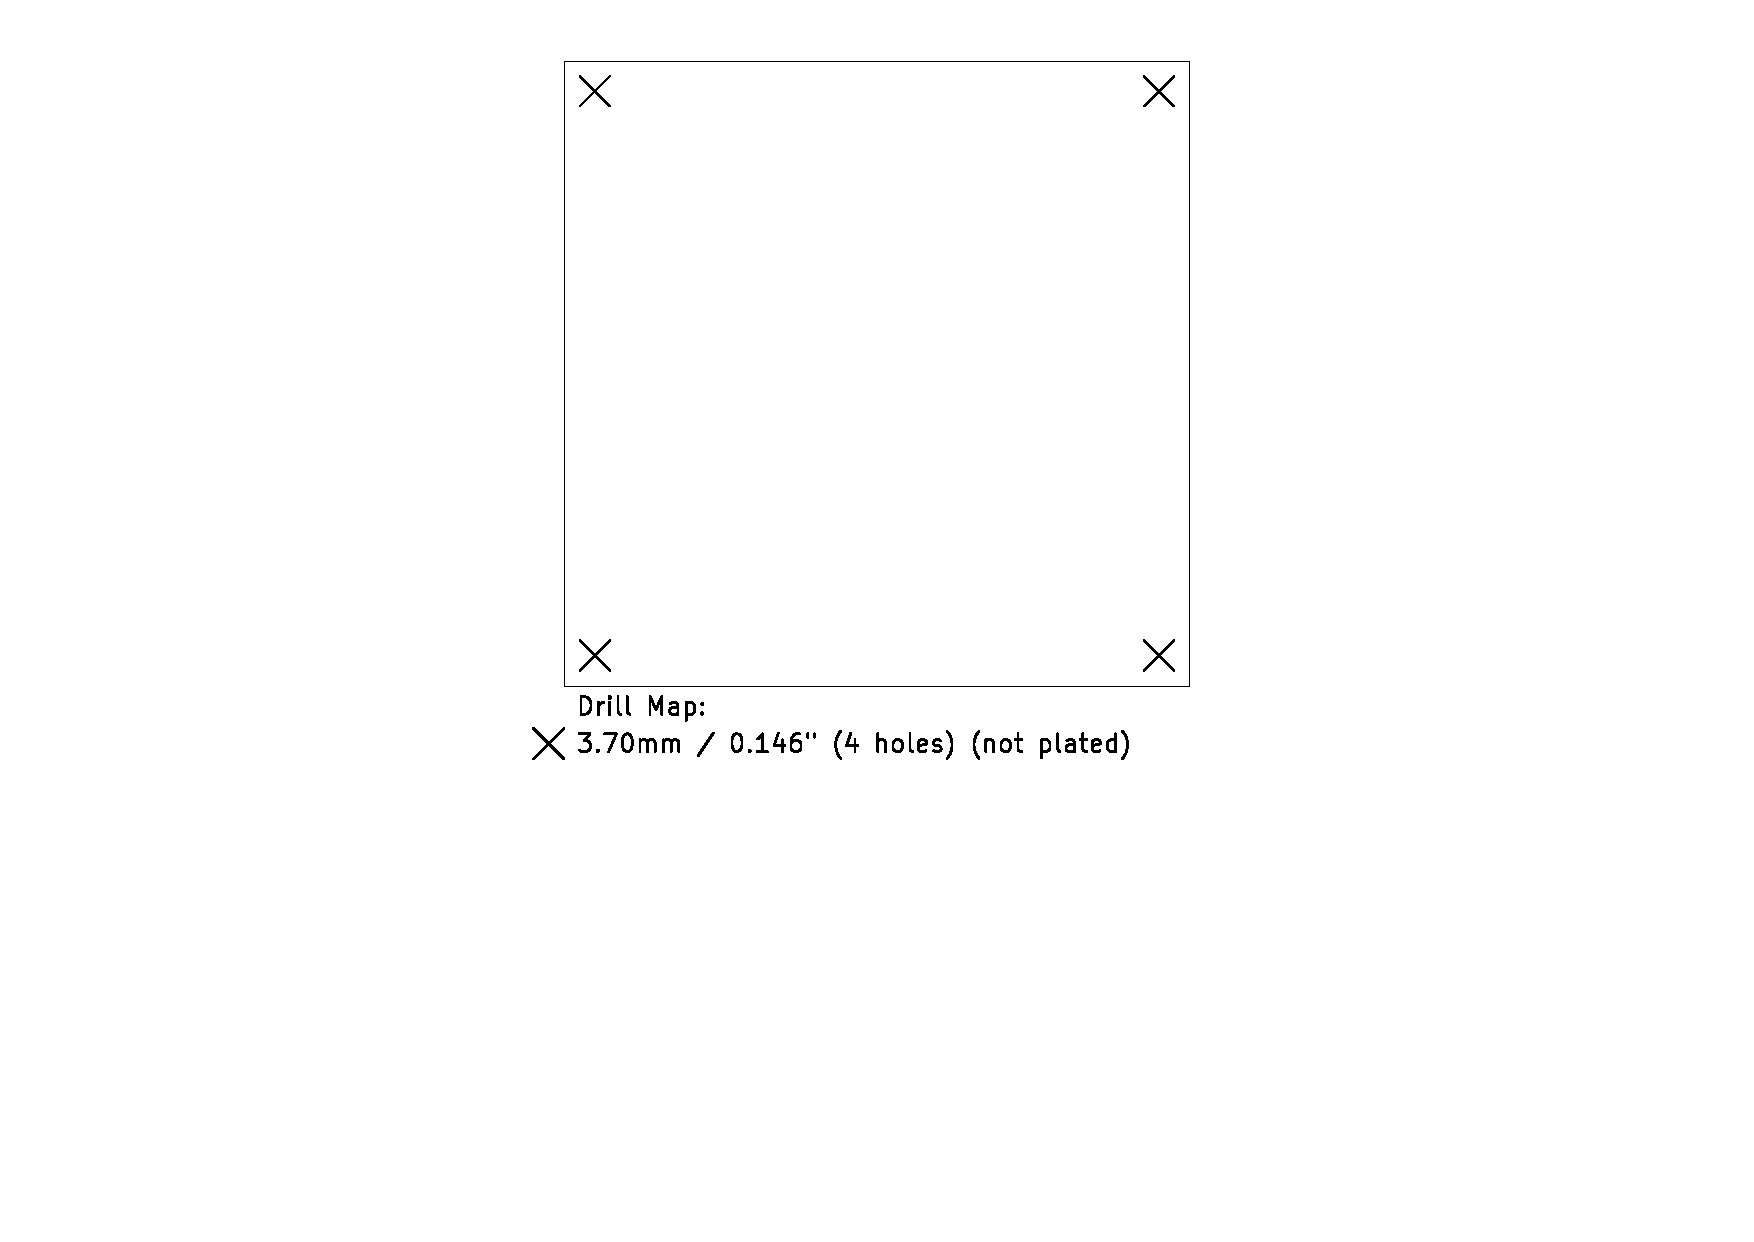
\includepdf[pages=-,pagecommand={},noautoscale=true,angle=90,addtotoc={1,subsection,2,Non-Plated
    Through-Hole Drill Map,fig:psu-NPTH-drl_map}]{../pcb/psu-NPTH-drl_map.pdf}
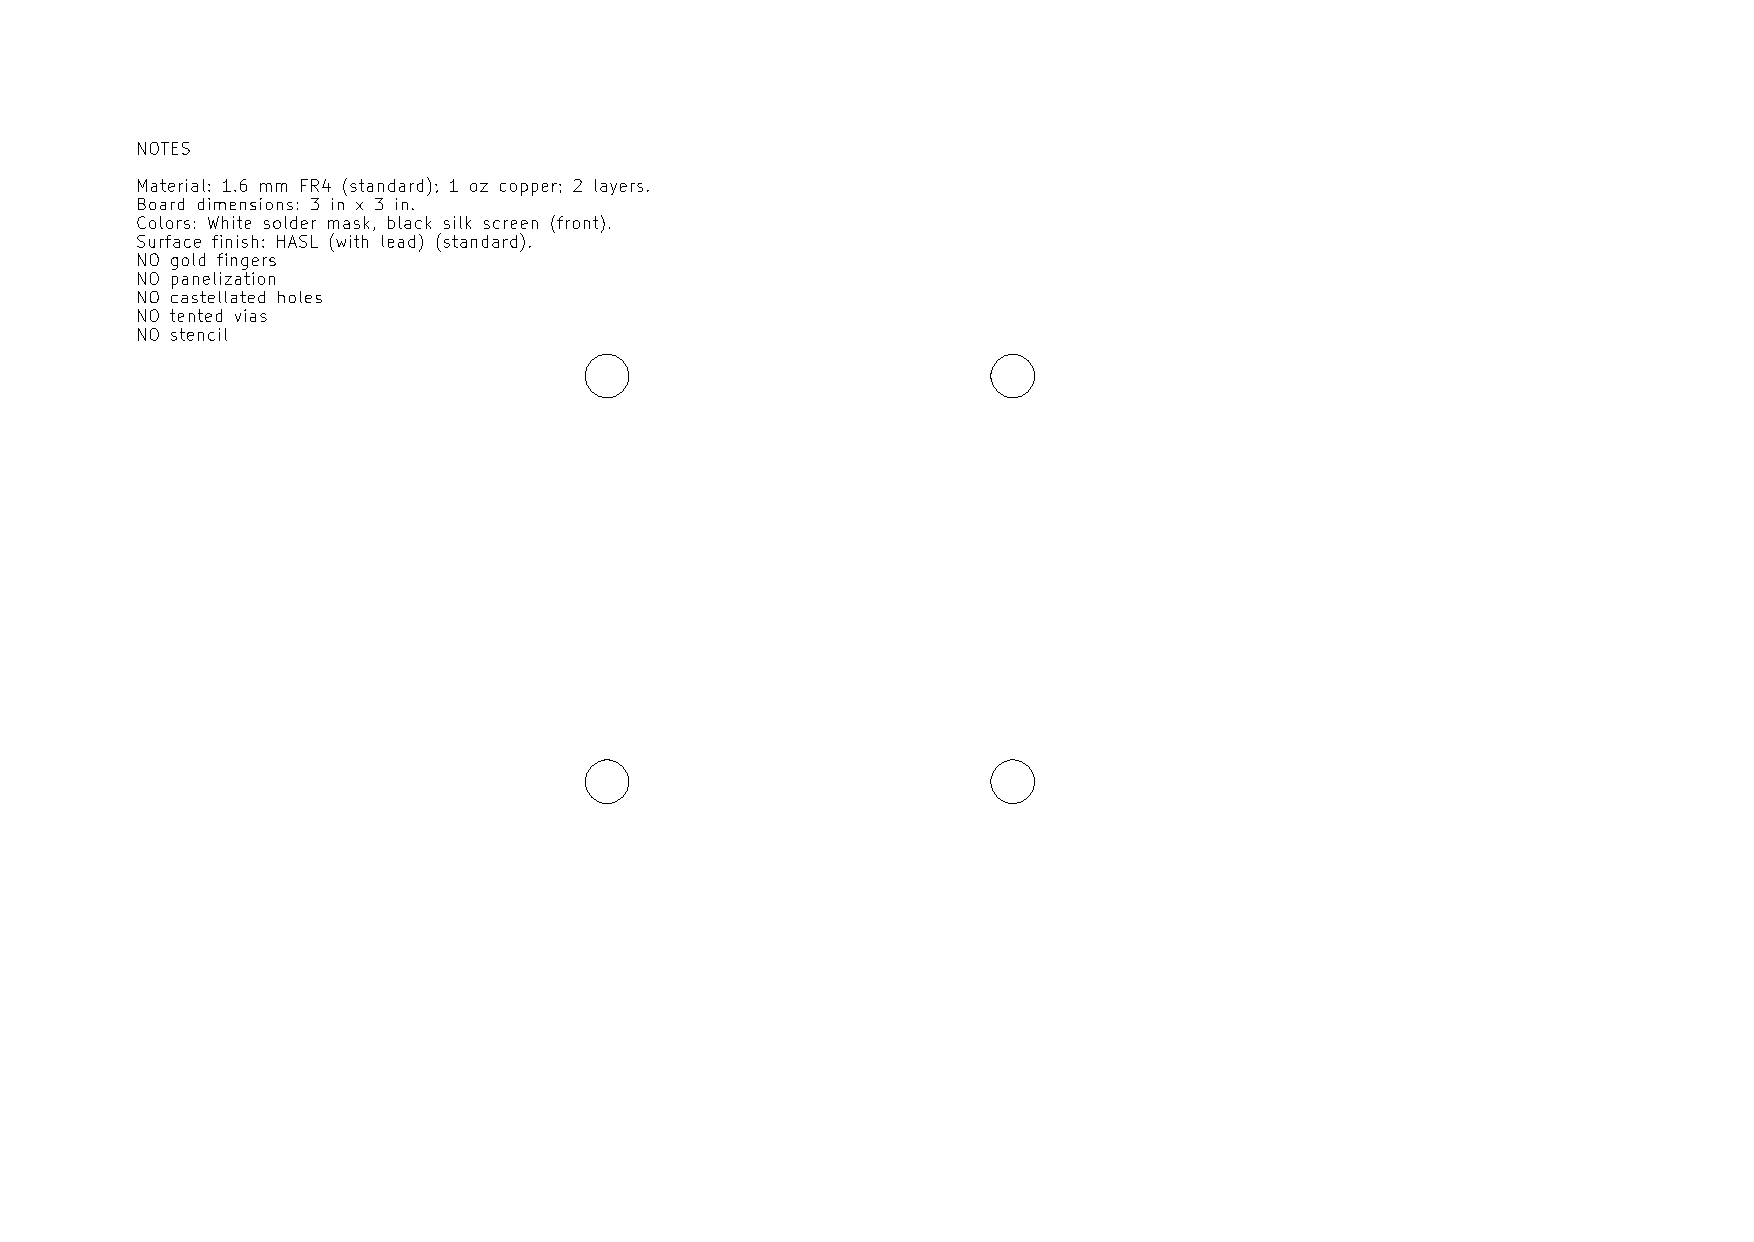
\includepdf[pages=-,pagecommand={},noautoscale=true,angle=90,addtotoc={1,subsection,2,User
    Comments,fig:psu-Cmts_User}]{../pcb/psu-Cmts_User.pdf}

\includepdf[pages=-,pagecommand={},noautoscale=true,angle=90,addtotoc={1,subsection,2,Edge
    Cuts (Board Outline),fig:psu-Edge_Cuts}]{../pcb/psu-Edge_Cuts.pdf}

% \section{Bill of Materials}

\begin{sidewaystable*}[ht]
  \caption[Bill of Materials]{Bill of materials with collated items. There are
  60 components total.}
  \resizebox{\linewidth}{!}{%
    \begin{tabular}{cclllll}
      \toprule
      \textbf{Item}          & \textbf{Qty}
      & \textbf{Reference(s)}           & \textbf{Value}                  &
      \textbf{LibPart}                          & \textbf{Footprint} \\
      \midrule
      1                      & 6                                                        & C1, C2, C5, C6, C7, C8 & 0u1                    & Device:C\_Small                  & Capacitor\_THT:C\_Disc\_D5.0mm\_W2.5mm\_P2.50mm                                                         \\
      2                      & 2                                                        & C3, C4                 & 10u                    & Device:C\_Small                  & Capacitor\_SMD:C\_1206\_3216Metric\_Pad1.42x1.75mm\_HandSolder                                          \\
      3                      & 2                                                        & D1, D2                 & LED\_RED               & Device:LED\_ALT                  & LED\_THT:LED\_D3.0mm                                                                                    \\
      4                      & 1                                                        & J1                     & Screw\_Terminal\_01x02 & Connector:Screw\_Terminal\_01x02 & TerminalBlock\_MetzConnect:TerminalBlock\_MetzConnect\_Type094\_RT03502HBLU\_1x02\_P5.00mm\_Horizontal  \\
      5                      & 1                                                        & J2                     & Barrel\_Jack           & Connector:Barrel\_Jack           & Connector\_BarrelJack:BarrelJack\_Horizontal                                                            \\
      6                      & 1                                                        & J3                     & Binding posts          & Connector\_Generic:Conn\_01x02   & psu-foot:Binding Posts                                                                                  \\
      7                      & 1                                                        & JP1                    & Min Lim                & Device:Jumper\_NO\_Small         & Connector\_PinHeader\_2.54mm:PinHeader\_1x02\_P2.54mm\_Vertical                                         \\
      8                      & 1                                                        & JP2                    & No limit               & Device:Jumper\_NO\_Small         & Connector\_PinHeader\_2.54mm:PinHeader\_1x02\_P2.54mm\_Vertical                                         \\
      9                      & 1                                                        & JP3                    & Preload                & Device:Jumper\_NO\_Small         & Connector\_PinHeader\_2.54mm:PinHeader\_1x02\_P2.54mm\_Vertical                                         \\
      10                     & 2                                                        & JP4, JP5               & Guard                  & Device:Jumper\_NO\_Small         & psu-foot:Guard\_Jumper                                                                                  \\
      11                     & 1                                                        & R1                     & 1R8                    & Device:R                         & Resistor\_SMD:R\_1206\_3216Metric\_Pad1.42x1.75mm\_HandSolder                                           \\
      12                     & 1                                                        & R2                     & 4R7                    & Device:R                         & Resistor\_SMD:R\_1206\_3216Metric\_Pad1.42x1.75mm\_HandSolder                                           \\
      13                     & 1                                                        & R3                     & 13R                    & Device:R                         & Resistor\_SMD:R\_1206\_3216Metric\_Pad1.42x1.75mm\_HandSolder                                           \\
      14                     & 1                                                        & R4                     & 27R                    & Device:R                         & Resistor\_SMD:R\_1206\_3216Metric\_Pad1.42x1.75mm\_HandSolder                                           \\
      15                     & 1                                                        & R5                     & 68R                    & Device:R                         & Resistor\_SMD:R\_1206\_3216Metric\_Pad1.42x1.75mm\_HandSolder                                           \\
      16                     & 2                                                        & R6, R14                & 100R                   & Device:R                         & Resistor\_SMD:R\_1206\_3216Metric\_Pad1.42x1.75mm\_HandSolder                                           \\
      17                     & 1                                                        & R7                     & 180R                   & Device:R                         & Resistor\_SMD:R\_1206\_3216Metric\_Pad1.42x1.75mm\_HandSolder                                           \\
      18                     & 4                                                        & R8, R10, R11, R12      & 1R0                    & Device:R                         & Resistor\_SMD:R\_1206\_3216Metric\_Pad1.42x1.75mm\_HandSolder                                           \\
      19                     & 1                                                        & R9                     & 2R2                    & Device:R                         & Resistor\_SMD:R\_1206\_3216Metric\_Pad1.42x1.75mm\_HandSolder                                           \\
      20                     & 1                                                        & R13                    & 39R                    & Device:R                         & Resistor\_SMD:R\_1206\_3216Metric\_Pad1.42x1.75mm\_HandSolder                                           \\
      21                     & 1                                                        & R15                    & 4k7                    & Device:R                         & Resistor\_THT:R\_Axial\_DIN0207\_L6.3mm\_D2.5mm\_P10.16mm\_Horizontal                                   \\
      22                     & 1                                                        & R16                    & 390R                   & Device:R                         & Resistor\_THT:R\_Axial\_DIN0207\_L6.3mm\_D2.5mm\_P10.16mm\_Horizontal                                   \\
      23                     & 1                                                        & R17                    & 1k5                    & Device:R                         & Resistor\_SMD:R\_1206\_3216Metric\_Pad1.42x1.75mm\_HandSolder                                           \\
      24                     & 1                                                        & R18                    & 1M                     & Device:R                         & Resistor\_SMD:R\_1206\_3216Metric\_Pad1.42x1.75mm\_HandSolder                                           \\
      25                     & 1                                                        & R19                    & 24k                    & Device:R                         & Resistor\_SMD:R\_1206\_3216Metric\_Pad1.42x1.75mm\_HandSolder                                           \\
      26                     & 2                                                        & R20, R26               & 1k                     & Device:R                         & Resistor\_SMD:R\_1206\_3216Metric\_Pad1.42x1.75mm\_HandSolder                                           \\
      27                     & 1                                                        & R21                    & 150k                   & Device:R                         & Resistor\_SMD:R\_1206\_3216Metric\_Pad1.42x1.75mm\_HandSolder                                           \\
      28                     & 1                                                        & R22                    & 1k                     & Device:R                         & Resistor\_THT:R\_Axial\_DIN0207\_L6.3mm\_D2.5mm\_P10.16mm\_Horizontal                                   \\
      29                     & 1                                                        & R23                    & 22R                    & Device:R                         & Resistor\_THT:R\_Axial\_DIN0207\_L6.3mm\_D2.5mm\_P10.16mm\_Horizontal                                   \\
      30                     & 2                                                        & R24, R25               & 10k                    & Device:R                         & Resistor\_SMD:R\_1206\_3216Metric\_Pad1.42x1.75mm\_HandSolder                                           \\
      31                     & 2                                                        & R27, R28               & 100R                   & Device:R                         & Resistor\_THT:R\_Axial\_DIN0207\_L6.3mm\_D2.5mm\_P10.16mm\_Horizontal                                   \\
      32                     & 1                                                        & RV1                    & 100R                   & Device:R\_POT\_US                & psu-foot:Trim\_pot\_Bourns\_TC33X-2-101E                                                                \\
      33                     & 1                                                        & RV2                    & 500k                   & Device:R\_POT\_US                & Potentiometer\_THT:Potentiometer\_Piher\_PC-16\_Single\_Horizontal                                      \\
      34                     & 1                                                        & RV3                    & 10k                    & Device:R\_POT\_US                & Potentiometer\_THT:Potentiometer\_Piher\_PC-16\_Single\_Horizontal                                      \\
      35                     & 1                                                        & RV4                    & 1k                     & Device:R\_POT\_US                & Potentiometer\_THT:Potentiometer\_Piher\_PC-16\_Single\_Horizontal                                      \\
      36                     & 1                                                        & RV5                    & 500k                   & Device:R\_POT\_US                & psu-foot:Trim\_pot\_Bourns\_TC33X-2-101E                                                                \\
      37                     & 2                                                        & SW1, SW2               & SW\_SP4T               & psu-sch:SW\_SP4T                 & psu-foot:SP4T\_CK\_SK-14D01-G-6                                                                         \\
      38                     & 1                                                        & SW3                    & Lever toggle           & Switch:SW\_SPST                  & psu-foot:SW\_SPST\_Lever\_Rubber                                                                        \\
      39                     & 1                                                        & U1                     & LM4040DBZ-2.5          & Reference\_Voltage:LM4040DBZ-2.5 & Package\_TO\_SOT\_SMD:SOT-23                                                                            \\
      40                     & 1                                                        & U2                     & LT3081                 & psu-sch:LT3081                   & Package\_SO:HTSSOP-16-1EP\_4.4x5mm\_P0.65mm\_EP3.4x5mm\_Mask3x3mm\_ThermalVias                          \\
      41                     & 1                                                        & U3                     & LM393                  & Comparator:LM393                 & Package\_SO:SOIC-8\_3.9x4.9mm\_P1.27mm                                                                  \\
      42                     & 1                                                        & U4                     & LM334M                 & Reference\_Current:LM334M        & Package\_SO:SOIC-8\_3.9x4.9mm\_P1.27mm                                                                  \\
      43                     & 2
      & U5, U6                 & LM317L\_TO92           &
      Regulator\_Linear:LM317L\_TO92   & Package\_TO\_SOT\_THT:TO-92\_Inline
      \\
      \bottomrule
  \end{tabular}}
\end{sidewaystable*}
\clearpage

\end{document}

